% ACL 2026 / BabyLM Workshop Paper
\documentclass[11pt,a4paper]{article}
\usepackage[review]{acl}
\usepackage{times}
\usepackage{latexsym}
\usepackage[T1]{fontenc}
\usepackage[utf8]{inputenc}
\usepackage{microtype}
\usepackage{graphicx}
\usepackage{booktabs}
\usepackage{amsmath}
\usepackage{amssymb}
\usepackage{hyperref}
\usepackage{placeins}
\usepackage{float}

% ---- Consistent method naming ----
\newcommand{\standardmlm}{Standard MLM}
\newcommand{\syntagmatic}{Syntagmatic}
\newcommand{\paradigmatic}{Paradigmatic}
\newcommand{\relayjoint}{Relay Joint}
\newcommand{\msd}[2]{#1{\scriptsize$\pm#2$}}
\newcommand{\bestmsd}[2]{\textbf{#1}{\scriptsize$\pm#2$}}

\title{Learning What Can Combine and What Can Substitute:\\
 Relational Inductive Biases for BabyLM Pretraining}

\author{Anonymous Submission}

\date{}

\begin{document}
\raggedbottom
\maketitle

\begin{abstract}
Language derives its productivity from syntagmatic relations of
combination and paradigmatic relations of choice. We introduce two
self-generated detached representation targets for masked language
modeling: Syntagmatic aligns selected positions with attention-weighted
contextual support, and Paradigmatic aligns them with centroids of
current input-embedding neighbors. The formal submission system,
\relayjoint{}, stages these targets in relation-specific slices,
retains a reduced Syntagmatic signal after syntax-level Paradigmatic
activation, and anchors entity representations during the middle of
training. No objective uses additional corpus data, external
annotation, or trainable parameters. Under the latest BabyLM~2026
nine-metric evaluation, a controlled seed-0 comparison yields Overall
scores of 39.69, 40.31, 40.20, and 40.94 for Standard MLM,
Syntagmatic, Paradigmatic, and Relay Joint. Relay Joint is 1.25 points
above its seed-matched baseline and obtains the highest score, with
large gains on BLiMP Supplement and smaller gains on several other
metrics. Entity Tracking and Reading decline. Because Relay Joint is
available here only for seed 0, we report no cross-seed standard
deviation, significance test, or universal improvement claim.
\end{abstract}

% =================================================================
\section{Introduction}
% =================================================================

Language is an economical, efficient, and flexible hierarchical
symbolic system. A finite inventory of linguistic units supports a
virtually unbounded range of expressions because these units are not
isolated: they participate together in syntagmatic relations of
combination and paradigmatic relations of choice. Syntagmatic relations
determine which units can combine to form larger
structures~\cite{saussure1916cours,firth1957synopsis}, whereas
paradigmatic relations organize the alternatives that may occupy the
same structural
position~\cite{saussure1916cours,halliday1961categories,harris1954distributional}.
Together, these axes support the hierarchical organization,
productivity, and generalization capacity of language.

This organization suggests a hypothesis for learning from limited
input. Learners cannot memorize every possible expression; they must
abstract structures and categories that transfer beyond observed
instances~\cite{tomasello2003constructing,bybee2010language}.
Combination relations provide regularities over how units form larger
patterns, while choice relations organize categories of fillers for a
shared position. If a language model is explicitly encouraged to
capture both kinds of regularity, it may rely less on memorizing
individual expressions and instead form reusable structures and
categories. We refer to this proposal as the \textbf{Relational
Efficiency Hypothesis}. It is a research hypothesis about
fixed-exposure generalization, not a claim of computational speed.

Masked language modeling (MLM)~\cite{devlin2019bert} already offers
implicit opportunities to learn both relations: predicting a missing
token requires sensitivity to context and lexical alternatives.
However, token-level cross-entropy directly supervises only the
identity of the gold token. It does not explicitly require the masked
representation to retain which contextual units support combination
at that position or which lexical units approximate a potential choice
class. We do not assume that standard MLM lacks these properties;
rather, we test whether explicit relational representation targets
provide a useful inductive bias when input is
limited~\cite{warstadt2023findings,hu2024babylm}.

We operationalize the two axes through detached, model-internal
targets at MLM-selected positions. \syntagmatic{} uses last-layer
attention to construct an attention-weighted target from eligible
visible context, approximating contextual support. \paradigmatic{}
uses the current input-embedding neighbors of the gold token to
construct a neighborhood centroid, approximating substitutional
choice. Neither objective adds corpus data, external annotation, or
trainable parameters. Training the targets alone and in the staged \relayjoint{} system
compares four seed-0 checkpoints under a shared backbone, corpus,
masking process, and exposure budget. The single-target systems isolate
the two relational biases; Relay Joint is the formal submission model
and follows the schedule saved with the formal v22 checkpoint.
Its latest nine-metric Overall is 40.94, compared with 39.69 for the
seed-matched Standard MLM baseline. Improvements are task-dependent,
and the single-seed result does not establish statistical significance
or general synergy.

Our contributions are:
\begin{enumerate}
 \item \textbf{Theory.} The Relational Efficiency Hypothesis connects
 syntagmatic--paradigmatic organization to language generalization
 under limited exposure.

 \item \textbf{Method.} Two self-generated, detached, and
 parameter-neutral relational targets approximate contextual
 combination and substitutional choice at MLM-selected positions,
 together with the staged Relay Joint schedule used by the submitted
 checkpoint.

 \item \textbf{Evidence.} A seed-matched comparison of Standard MLM,
 Syntagmatic, Paradigmatic, and Relay Joint under the current official
 nine-metric evaluation, supplemented by checkpoint trajectories and
 a seed-0 representation analysis.
\end{enumerate}

\begin{figure*}[t]
 \centering
 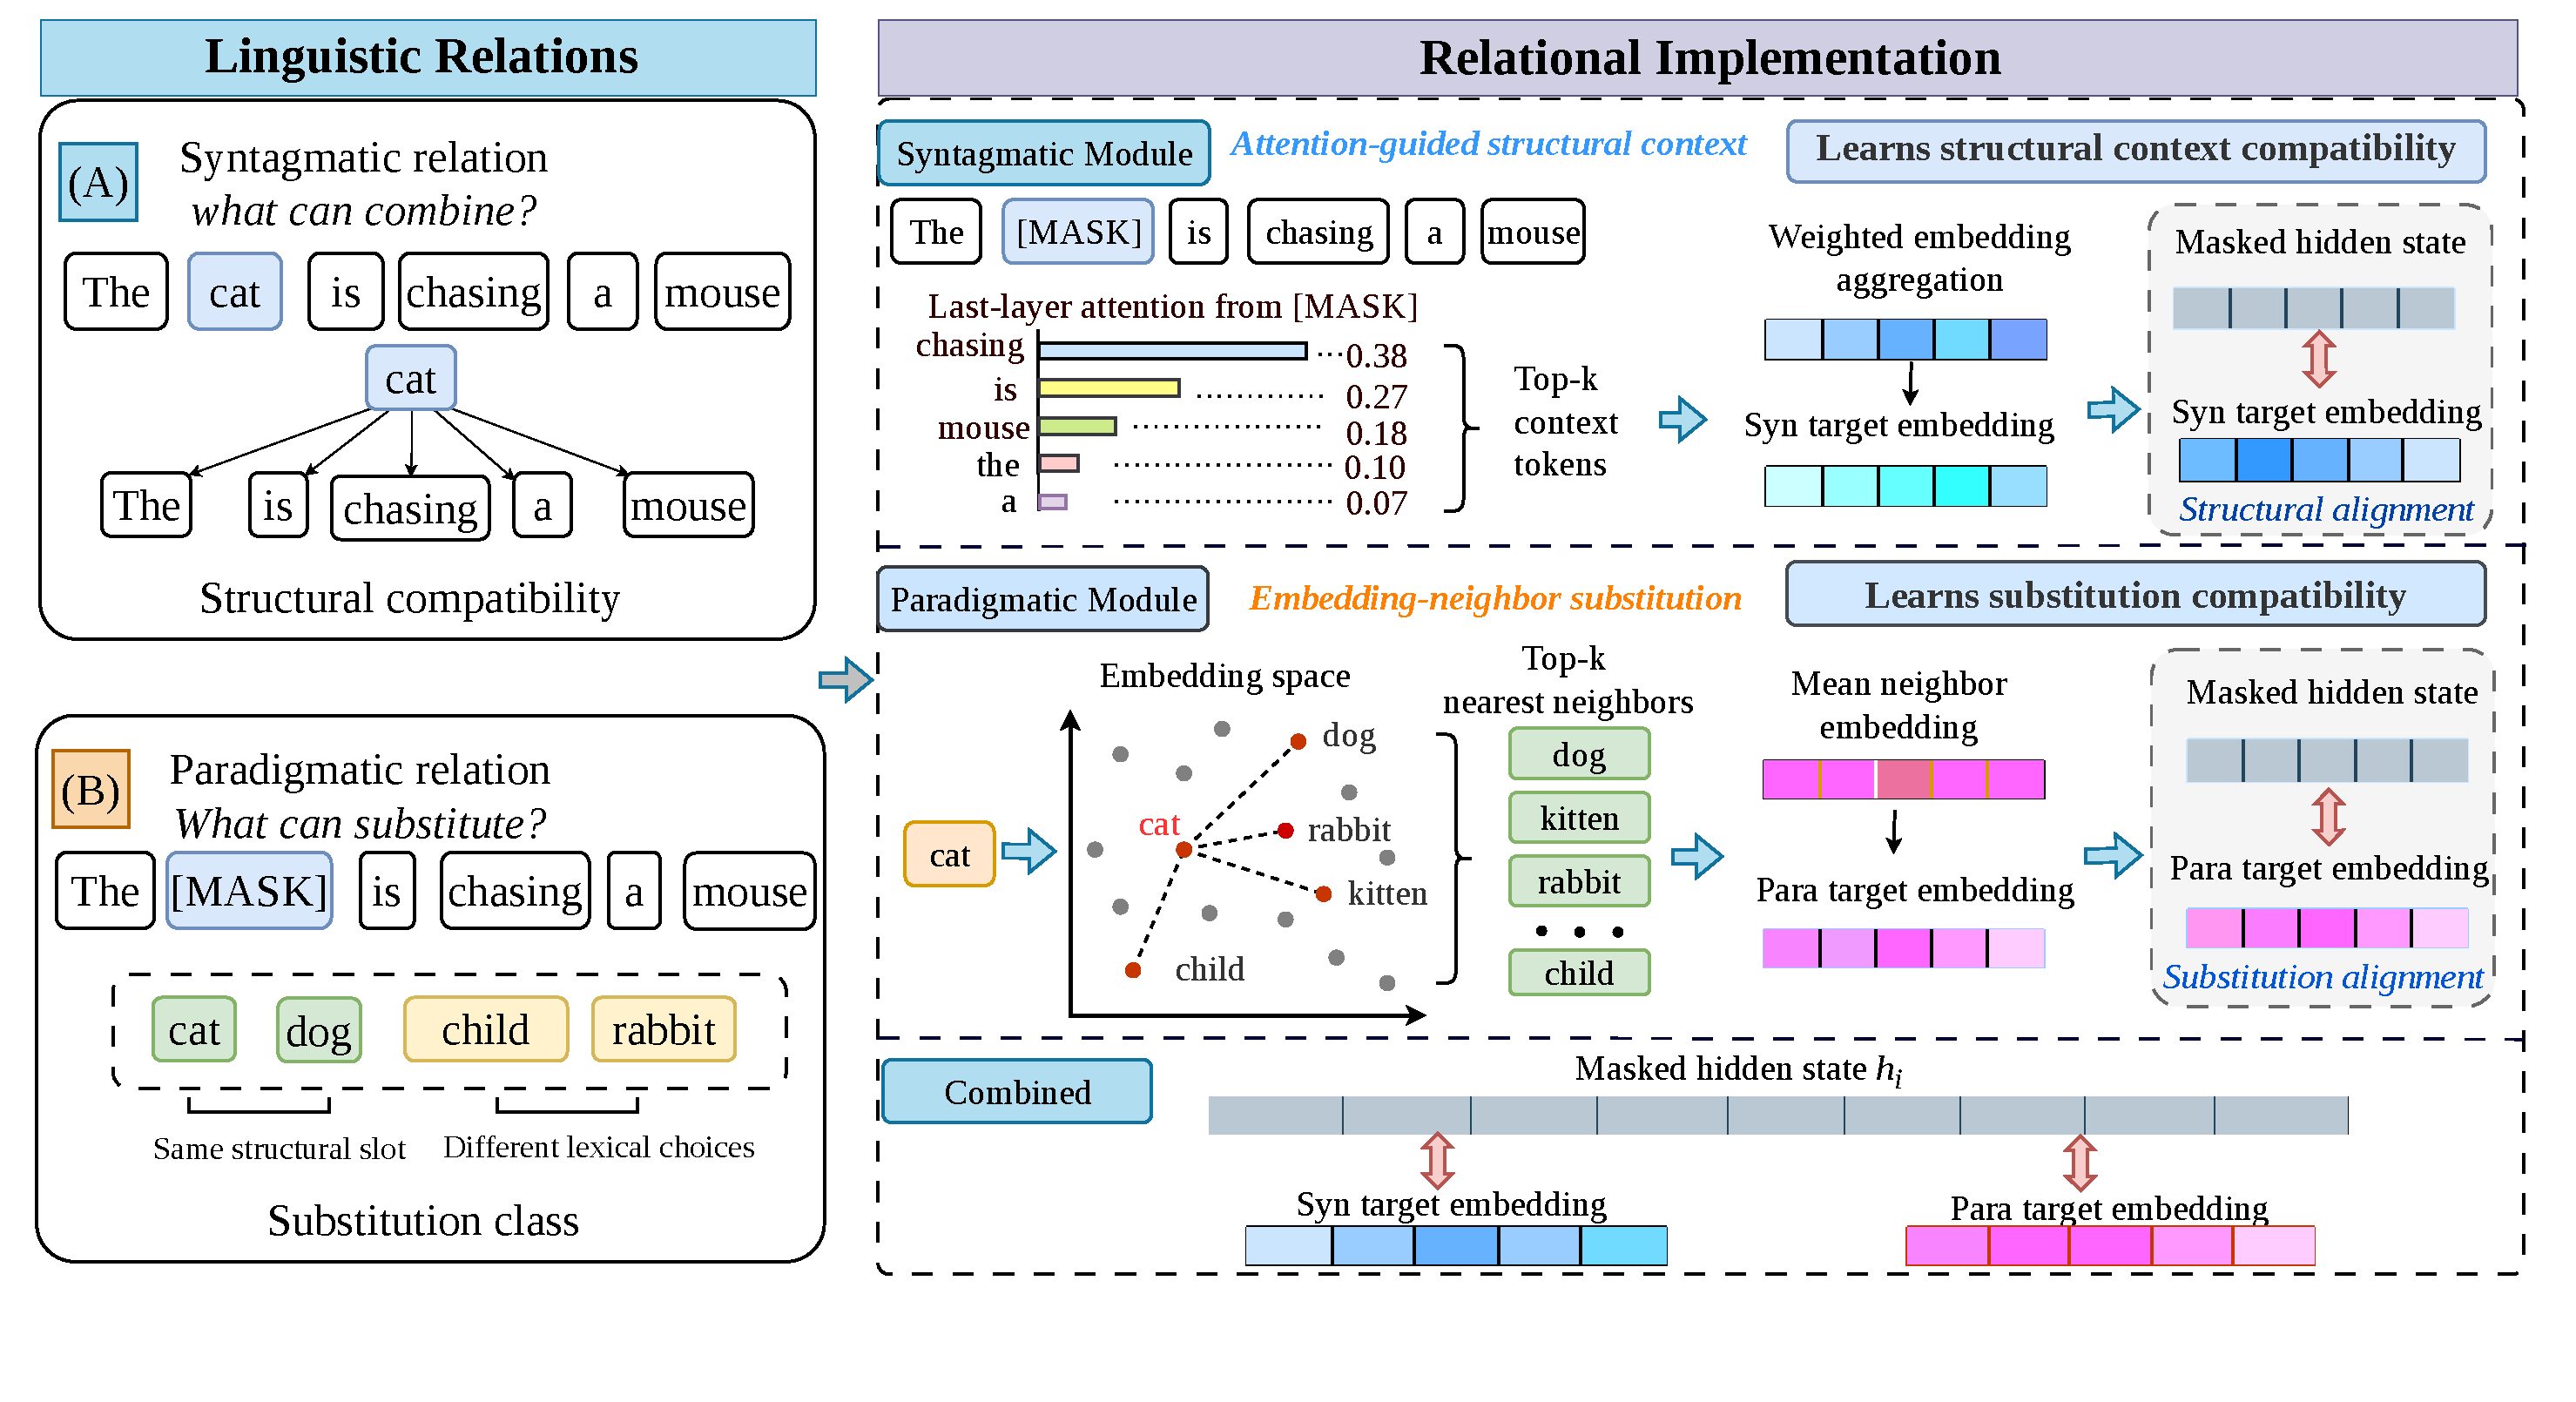
\includegraphics[width=\textwidth]{figures/yyw0712-2-5.drawio.pdf}
 \caption{Overview of the relational pretraining framework. The four compared systems share the same backbone, data, and training schedule; they differ only in which relational targets are active at MLM-selected positions.}
 \label{fig:overview}
\end{figure*}

% =================================================================
\section{Related Work}
% =================================================================

\subsection{Syntagmatic and Paradigmatic Organization}

\citet{saussure1916cours} distinguished syntagmatic relations among
units combined in sequence from associative, later paradigmatic,
relations among alternatives \emph{in absentia}.
\citet{halliday1961categories} recast this contrast as structure
(chain) and system (choice), while \citet{harris1954distributional}
used distributional equivalence to characterize substitution classes.
\citet{sahlgren2008distributional} connected the distinction to
distributional representation: direct co-occurrence tends to emphasize
syntagmatic association, whereas similarity of contexts tends to
emphasize paradigmatic association.

Usage-based and construction-based theories further explain how
repeated instances can support schemas with structurally constrained
slots~\cite{tomasello2003constructing,bybee2010language,goldberg2006constructions}.
Word-association studies document related contrasts in human
responses~\cite{brown1960word,ervin1961changes,entwisle1964syntactic}.
These traditions motivate the relational axes, but our continuous
targets are model-internal approximations rather than symbolic
linguistic structures. The unresolved question is whether both axes
can be operationalized as useful inductive biases for pretraining from
limited exposure.

\subsection{Relational Signals in Language Models}

\citet{sun2015learning} modeled syntagmatic and paradigmatic relations
in static embeddings, while \citet{mickus2024language} interpreted MLM
through the paradigmatic axis. Lexical-substitution work instead
generates or ranks context-appropriate substitutes with contextual
models~\cite{melamud2016context2vec,zhou2019bertbased} or human
annotations~\cite{lee2021swords}. Our objective neither generates
substitutes nor uses labeled substitute sets; it treats the current
input-embedding neighborhood as a distributional approximation.

Attention analyses provide another source of relational evidence:
individual heads can correlate with syntactic
relations~\cite{clark2019what}, although attention is not a guaranteed
explanation or syntactic ground truth~\cite{jain2019attention}.
Similarly, distributional co-occurrence explains much but not all MLM
generalization~\cite{sinha2021masked,chiang2023distributional}. Unlike
post-hoc analyses, both objectives here are generated from internal
model signals and train MLM-selected contextual hidden states. The gap
we address is whether these approximate signals can serve as training
biases rather than merely describe representations after training.

\subsection{Data-Constrained Pretraining}

The BabyLM challenge~\cite{warstadt2023findings,hu2024babylm,charpentier2025findings}
tests language learning under tightly constrained input. Existing work
has improved such training through architectural
changes~\cite{huebner2021babyberta}, alternative or combined training
objectives~\cite{charpentier2024gpt}, adaptive masking
strategies~\cite{edman2025mask}, and data
organization~\cite{haga2024babylm}. These approaches show several
routes to stronger limited-data models, but do not isolate the effect
of the two relational axes on the representation at a masked position.
Our comparison therefore fixes the corpus, corruption process,
backbone, and cumulative exposure, changing only the detached
relational targets applied to MLM-selected hidden states.

% =================================================================
\section{Method}
\label{sec:method}
% =================================================================

Let $x_i$ be the gold token at an MLM-selected position $i$, and let
$\mathbf{h}_i\in\mathbb{R}^{384}$ be its final-layer contextual hidden
state before the MLM prediction head. Standard MLM minimizes token
cross-entropy $\mathcal{L}_{\mathrm{MLM}}$. Both relational objectives
construct a target from signals already available inside the model and
apply stop-gradient to that target. Consequently, an auxiliary target
cannot move simply to reduce its own loss; the relational gradient
updates the model through the contextual hidden-state branch. Neither
objective requires new training data or introduces additional
trainable parameters.

\subsection{Syntagmatic Alignment}
\label{sec:syntagmatic}

Syntagmatic relations concern how linguistic units combine within an
expression. We approximate this relation by asking which visible
context positions the model's final attention layer treats as support
for an MLM-selected position. Specifically, we average last-layer
attention across all 12 heads. We exclude the target position, padding,
\texttt{[CLS]}, \texttt{[SEP]}, \texttt{[MASK]}, and every other
MLM-selected position, then select the top $K=8$ remaining visible
positions. Let $\mathcal{A}_i$ be this set and
$\widetilde{\alpha}_{ij}$ the selected attention logits normalized by
a softmax over $\mathcal{A}_i$. Using embeddings of the original,
uncorrupted input tokens, the target is

\begin{equation}
\mathbf{s}_i =
\operatorname{sg}\!\left(
\sum_{j\in\mathcal{A}_i}
\widetilde{\alpha}_{ij}\mathbf{e}(x_j)
\right),
\label{eq:syntagmatic_target}
\end{equation}

where $\operatorname{sg}$ denotes stop-gradient. The position-level
loss is

\begin{equation}
\ell_{\mathrm{syn},i}=1-\cos(\mathbf{h}_i,\mathbf{s}_i).
\label{eq:syntagmatic_alignment}
\end{equation}

The loss acts on the complete 384-dimensional hidden state. It is
weighted by $\lambda_{\mathrm{syn}}=5\times10^{-4}$ and becomes active
after approximately $9.2\%$ of training. MLM-selected entity tokens
and tokens deemed invalid by the fixed vocabulary lookup do not
receive this target. This target approximates prediction-relevant
contextual support; it is not an explicit dependency representation.

\subsection{Paradigmatic Alignment}
\label{sec:paradigmatic}

Paradigmatic relations concern the alternatives that can occupy a
shared structural position. Because the training data provide no
explicit substitution sets, we approximate this relation using the
gold token's neighborhood in the model's current input embedding
space. For each eligible MLM-selected position, we find the $K=8$
vocabulary items with highest cosine similarity to the gold token,
excluding the gold token itself:

\begin{equation}
\mathcal{N}_i =
\operatorname{TopK}_{v\neq x_i}
\cos\left(\mathbf{e}(x_i),\mathbf{e}(v)\right).
\label{eq:paradigmatic_neighbors}
\end{equation}

The target and loss are

\begin{align}
\mathbf{p}_i & =
\operatorname{sg}\!\left(
\frac{1}{K}\sum_{v\in\mathcal{N}_i}\mathbf{e}(v)
\right),
\label{eq:paradigmatic_target}\\
\ell_{\mathrm{para},i} & =
1-\cos(\mathbf{h}_i,\mathbf{p}_i).
\label{eq:paradigmatic_alignment}
\end{align}

The neighbor centroid is aligned with the full 384-dimensional hidden
state; no content projection is used. For syntax tokens, the loss
weight is $5\times10^{-5}$ and activation begins after approximately
$55.2\%$ of training. For content tokens, the weight is $10^{-6}$ and
activation begins at $99\%$, so the loss is active only during the
final $1\%$. Entity and reading-sensitive tokens do not receive a
Paradigmatic loss. The fixed vocabulary categories and their lookup
priority are detailed in Appendix~\ref{app:training-config}.
Embedding neighborhoods are distributional approximations to
potential alternatives, not guaranteed grammatical substitutes in a
particular context.

\subsection{Relay Joint Objective}
\label{sec:relay-joint}

The formal submission model combines the two targets with a staged,
fixed-subspace schedule. The Syntagmatic loss is applied to dimensions
0--255 of the contextual state and target, while the Paradigmatic loss
is applied to dimensions 256--383. These are fixed coordinate slices,
not learned projections. Standard MLM continues to use the complete
hidden state, and the auxiliary design adds no trainable parameters.

Syntagmatic supervision begins after approximately $9.2\%$ of
optimization with weight $5\times10^{-4}$. Syntax-token Paradigmatic
supervision begins after approximately $18.4\%$ with weight
$5\times10^{-5}$. From that point onward, the Syntagmatic
per-position weight on syntax tokens is retained at $10\%$ of its
earlier strength rather than removed. Content-token Paradigmatic
supervision has weight $10^{-6}$ and begins at $99\%$, so it is
active only in the final $1\%$ of training. Entity and
reading-sensitive tokens receive no Paradigmatic loss, and entity
tokens receive no Syntagmatic loss.

Relay Joint also applies an entity representation anchor to eligible
MLM-selected entity tokens from approximately $9.2\%$ until
$60\%$ of training:
\begin{equation}
\ell_{\mathrm{ent},i}
=1-\cos\left(
\mathbf{h}_i,
\operatorname{sg}(\mathbf{e}(x_i))
\right).
\label{eq:entity-anchor}
\end{equation}
The anchor uses the complete 384-dimensional hidden state and has
weight $2.5\times10^{-4}$.

Let $P_{0:256}$ and $P_{256:384}$ select the two fixed coordinate
slices, let each $\mathcal{L}$ be averaged over its eligible
positions, and let $g(t)$ denote the corresponding progress gate.
The Relay Joint objective is
\begin{align}
\mathcal{L}(t)={}&\mathcal{L}_{\mathrm{MLM}}
+\lambda_{\mathrm{syn}}g_{\mathrm{syn}}(t)
\mathcal{L}_{\mathrm{syn}}^{0:256}
\nonumber\\
&+\lambda_{\mathrm{para,syn}}g_{\mathrm{para,syn}}(t)
\mathcal{L}_{\mathrm{para,syn}}^{256:384}
\nonumber\\
&+\lambda_{\mathrm{para,cont}}g_{\mathrm{para,cont}}(t)
\mathcal{L}_{\mathrm{para,cont}}^{256:384}
\nonumber\\
&+\lambda_{\mathrm{ent}}g_{\mathrm{ent}}(t)
\mathcal{L}_{\mathrm{ent}} .
\label{eq:relay-loss}
\end{align}
No content projection, learned router, extra corpus, or additional
trainable module is enabled. The single-target systems retain their
original full-384 losses; Table~\ref{tab:schedule} therefore
summarizes implementation differences rather than a $2\times2$
factorial identity.

\begin{table}[t]
\centering
\footnotesize
\setlength{\tabcolsep}{1.8pt}
\begin{tabular}{lcccc}
\toprule
Method & Syn & Para & Rel. rep. & Ent. anchor \\
\midrule
\standardmlm & No & No & -- & No \\
\syntagmatic & Yes & No & Full 384 & No \\
\paradigmatic & No & Yes & Full 384 & No \\
\relayjoint & Yes & Yes & Syn 256 / Para 128 & Yes \\
\bottomrule
\end{tabular}
\caption{The four seed-0 systems. Relay Joint uses fixed slices
0--255 for Syntagmatic alignment and 256--383 for Paradigmatic
alignment; MLM prediction always uses the full state.}
\label{tab:schedule}
\end{table}

% =================================================================
\section{Experimental Setup}
% =================================================================

\subsection{Data and Training}
\label{sec:data-training}

All configurations use the official BabyLM~2026 Strict-Small corpus
released on Hugging Face\footnote{\url{https://huggingface.co/datasets/BabyLM-community/BabyLM-2026-Strict-Small}}
and the shared setup in Table~\ref{tab:shared-training}
\citep{choshen2026babylmturns4papers}. The corpus contains approximately
10M words. Models train for 10 epochs, with cumulative exposure no
greater than 100M words. The comparison reported here uses seed 0 for
all four systems because the formal Relay Joint result is the specified
v22-s0 submission checkpoint; no other v22 seed is included. All four
systems have 34,677,952 parameters. Parameter-neutral means that the
auxiliary objectives introduce no trainable parameters, although they
do add target-construction and loss-computation cost.

\begin{table}[t]
\centering
\small
\setlength{\tabcolsep}{4pt}
\begin{tabular}{@{}p{0.34\columnwidth}p{0.60\columnwidth}@{}}
\toprule
\textbf{Setting} & \textbf{Value} \\
\midrule
Backbone & DeBERTa-v2~\cite{he2021deberta}, 12 layers, 12 heads \\
Hidden / FFN size & 384 / 1280 \\
Tokenizer & SentencePiece, 40,000 tokens \\
Parameters & 34,677,952 \\
Sequence length & 64 (epochs 1--5); 256 (epochs 6--10) \\
MLM probability & Linear $0.40\rightarrow0.15$ \\
Replacement & 80\% mask, 10\% random, 10\% unchanged \\
Optimizer & LAMB~\cite{you2020lamb} \\
Peak learning rate & 0.007 \\
Schedule & 1\% warmup, cosine decay \\
Batch size & 256 \\
\bottomrule
\end{tabular}
\caption{Shared backbone and training configuration.}
\label{tab:shared-training}
\end{table}

\subsection{Evaluation}
\label{sec:evaluation}

We use the official BabyLM~2026 evaluation pipeline at commit
\texttt{3d57ddc8c40e}\footnote{The full commit hash is reported in
Appendix~\ref{app:reproduction}; repository:
\url{https://github.com/babylm-org/babylm-eval}.}
\citep{choshen2026babylmturns4papers}. Conventional NLP Performance
contains seven top-level metrics: BLiMP, BLiMP Supplement, EWoK,
Entity Tracking, COMPS, GlobalPIQA, and (Super)GLUE. Entity Tracking is
evaluated by whether the model assigns the highest probability to the
correct continuation rather than through free-form generation.
GlobalPIQA evaluates English physical commonsense reasoning over its
parallel and non-parallel subsets using the official scorer.
(Super)GLUE is the macro-average of BoolQ, MultiRC, RTE, WSC, MRPC,
QQP, and MNLI; MRPC and QQP use binary F1, and the other five tasks use
accuracy.

Human-likeness and Development contains Reading and Age of Acquisition
(AoA). Reading is $100$ times the mean normalized $\Delta R^2$ for
self-paced reading and eye tracking. AoA is $100$ times the Pearson
correlation between model-implied and child acquisition ages; the
pipeline sets this score to zero when $p>0.1$. Thus AoA can be negative.

\subsection{Reporting and Aggregation}
\label{sec:reporting}

Writing $B,S,E,T,C,G,L,R,A$ for the nine top-level metrics in the
order above, and $\mathcal{M}_9=\{B,S,E,T,C,G,L,R,A\}$, the
reported aggregates are
\begin{align}
\mathrm{NLP\ Avg} &= \frac{B+S+E+T+C+G+L}{7},\\
\mathrm{Human\ Avg} &= \frac{R+A}{2},\\
\mathrm{Overall} &= \frac{\sum_{m\in\mathcal{M}_9}m}{9}.
\label{eq:evaluation-aggregates}
\end{align}
Overall is therefore the direct macro-average of the nine top-level
metrics, not the mean of the two group averages. GlobalPIQA is the
official aggregate of its parallel and non-parallel subsets; Reading is
the official aggregate of self-paced reading and eye tracking; and
(Super)GLUE is the seven-task macro-average described above. We report
the seed-0 value for each method. With one run per method in this
comparison, sample standard deviations, paired significance tests, and
claims about consistency across seeds are unavailable.

% =================================================================
\section{Results}
% =================================================================

\subsection{Main Results}
\label{sec:main-results}

Tables~\ref{tab:nlp-results} and~\ref{tab:human-results} report the
full seed-0 evaluation, ordered by experimental condition rather than
rank. Both single-target systems improve Overall relative to Standard
MLM: Syntagmatic reaches 40.31 ($+0.62$), and Paradigmatic reaches
40.20 ($+0.51$). Relay Joint obtains the highest Overall, 40.94, a
$+1.25$ change from its seed-matched baseline. These are single-run
differences and do not establish cross-seed stability, statistical
significance, or general synergy.

\begin{table*}[t]
\centering
\scriptsize
\setlength{\tabcolsep}{3.2pt}
\renewcommand{\arraystretch}{1.12}
\begin{tabular}{lcccccccc}
\toprule
Method & BLiMP & B-Supp & EWoK & Entity & COMPS & GlobalPIQA & (Super)GLUE & NLP Avg \\
\midrule
\standardmlm & 66.80 & 58.57 & 51.39 & \textbf{22.53} & 51.90 & 35.13 & 64.82 & 50.16 \\
\syntagmatic & 67.56 & 60.37 & 49.10 & 20.84 & \textbf{52.50} & \textbf{38.62} & \textbf{67.52} & 50.93 \\
\paradigmatic & 67.13 & 62.30 & 52.28 & 21.67 & 52.22 & 34.62 & 65.78 & 50.86 \\
\relayjoint & \textbf{67.84} & \textbf{65.21} & \textbf{53.00} & 21.47 & 52.24 & 37.59 & 65.29 & \textbf{51.81} \\
\bottomrule
\end{tabular}
\caption{Conventional NLP Performance for seed 0. Bold marks the
highest value in each column.}
\label{tab:nlp-results}
\end{table*}

\begin{table}[t]
\centering
\small
\setlength{\tabcolsep}{3pt}
\begin{tabular}{lcccc}
\toprule
Method & Reading & AoA & Human Avg & Overall \\
\midrule
\standardmlm & 6.03 & \textbf{0.00} & 3.01 & 39.69 \\
\syntagmatic & \textbf{6.29} & \textbf{0.00} & \textbf{3.15} & 40.31 \\
\paradigmatic & 5.81 & \textbf{0.00} & 2.91 & 40.20 \\
\relayjoint & 5.83 & \textbf{0.00} & 2.92 & \textbf{40.94} \\
\bottomrule
\end{tabular}
\caption{Human-likeness and Overall for seed 0. Overall is the
macro-average of all nine top-level metrics, not an average of the two
group averages.}
\label{tab:human-results}
\end{table}

\subsection{Task-level Patterns}
\label{sec:task-patterns}

Compared with Standard MLM, Relay Joint improves six of nine
top-level metrics: BLiMP ($+1.04$), BLiMP Supplement ($+6.64$), EWoK
($+1.61$), COMPS ($+0.34$), GlobalPIQA ($+2.46$), and (Super)GLUE
($+0.47$). AoA is unchanged at zero. Entity Tracking decreases by
$1.06$, and Reading decreases by $0.20$. The aggregate advantage
therefore reflects strong gains on a subset of categories rather than
uniform improvement.

The two single-target systems also differ by task. Syntagmatic is
strongest on COMPS, GlobalPIQA, (Super)GLUE, Reading, Human Average,
and among the two single-target Overall scores. Paradigmatic is
stronger on BLiMP Supplement and EWoK. Relay Joint exceeds each
single-target Overall in this seed, but one seed cannot determine
whether the staged objectives are reliably complementary.

\begin{figure*}[t]
\centering
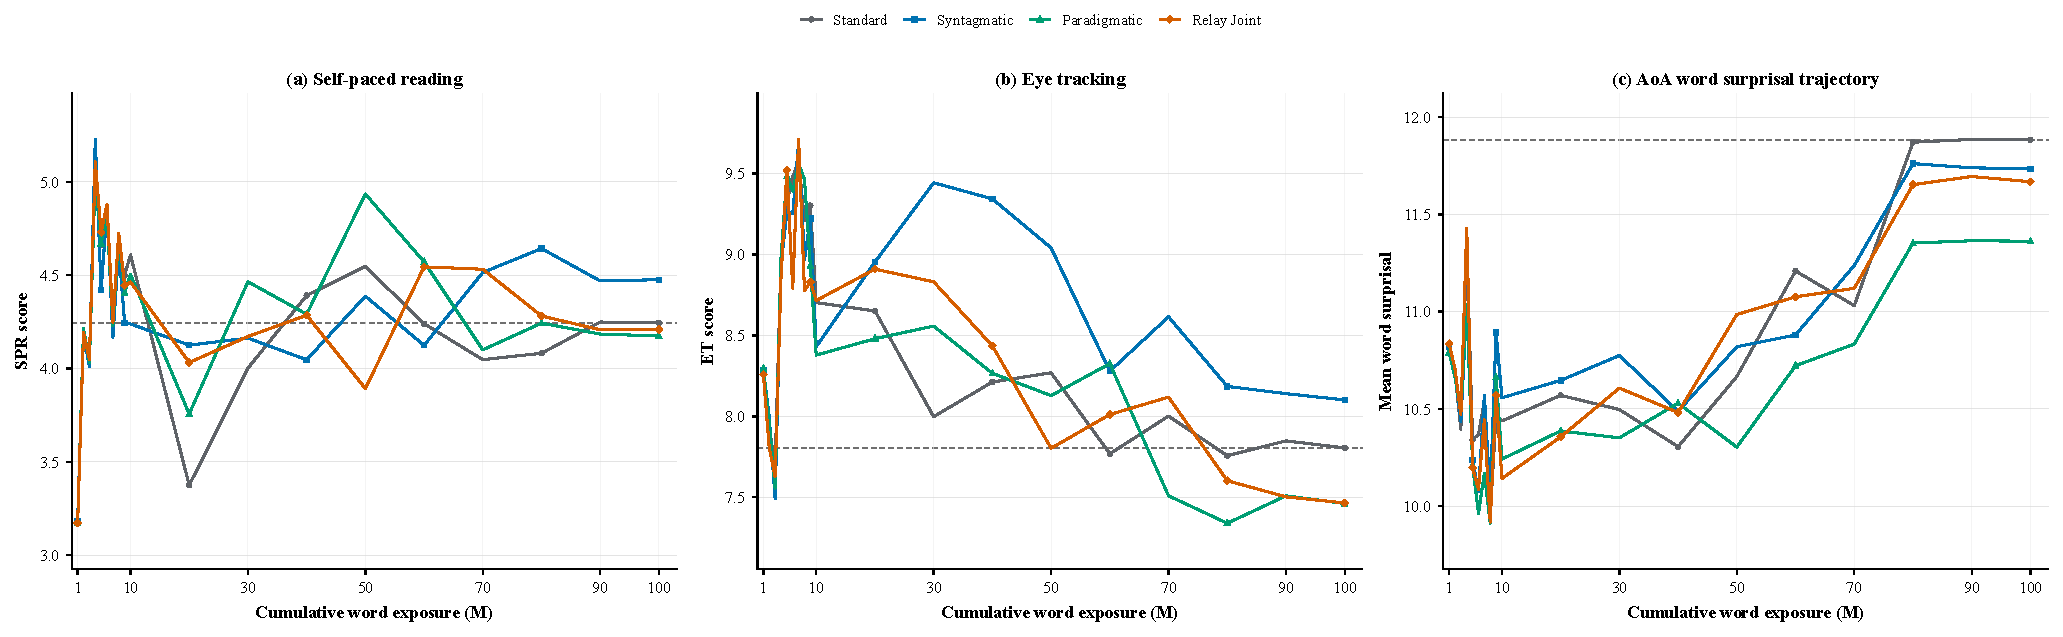
\includegraphics[width=\textwidth]{figures/figure2_reading_aoa_v22_s0.pdf}
\caption{Seed-0 Reading and AoA trajectories across training
checkpoints for the four evaluated systems. The Reading panels show
the official self-paced-reading and eye-tracking checkpoint scores.
The AoA panel shows mean target-word surprisal (lower is better), not
the official final AoA correlation used in Table~\ref{tab:human-results}.
Lines are single runs and therefore have no uncertainty bands.}
\label{fig:reading-aoa}
\end{figure*}

% =================================================================
\section{Analysis and Discussion}
\label{sec:analysis}
% =================================================================

We use targeted probes to ask whether the trained representations show
properties encouraged by the relational objectives. The Paradigmatic
probe was rerun for the exact seed-0 checkpoints in the main
comparison, including Relay Joint. The Syntagmatic diagnostics are a
separate three-seed single-module analysis of Standard MLM and
Syntagmatic only. Probes are not general quality metrics and cannot
by themselves explain downstream changes. Details appear in
Appendix~\ref{app:representation-analysis}.

\subsection{Paradigmatic Neighborhood Alignment}

For eligible masked syntax-token instances, we ask whether the hidden
state retrieves the correct gold-token neighbor centroid among 64
candidates (one correct target and 63 controls). Figure
\ref{fig:contextual-alignment} reports differences from the same
seed-0 Standard MLM checkpoint. In the full 384-dimensional state,
Paradigmatic changes alignment margin by $+0.0242$ and MRR by
$+0.0845$; Relay Joint changes them by $+0.0477$ and $+0.1445$.
For Relay Joint, the designated Paradigmatic slice has positive
differences ($+0.0877$ margin; $+0.1128$ MRR), but the complete-state
result is the primary representation-level comparison. The Syn-256
and Para-128 coordinates are fixed training slices, not discovered
latent subspaces. Because these are seed-0 results, no variance or
significance is reported.

\begin{figure}[t]
\centering
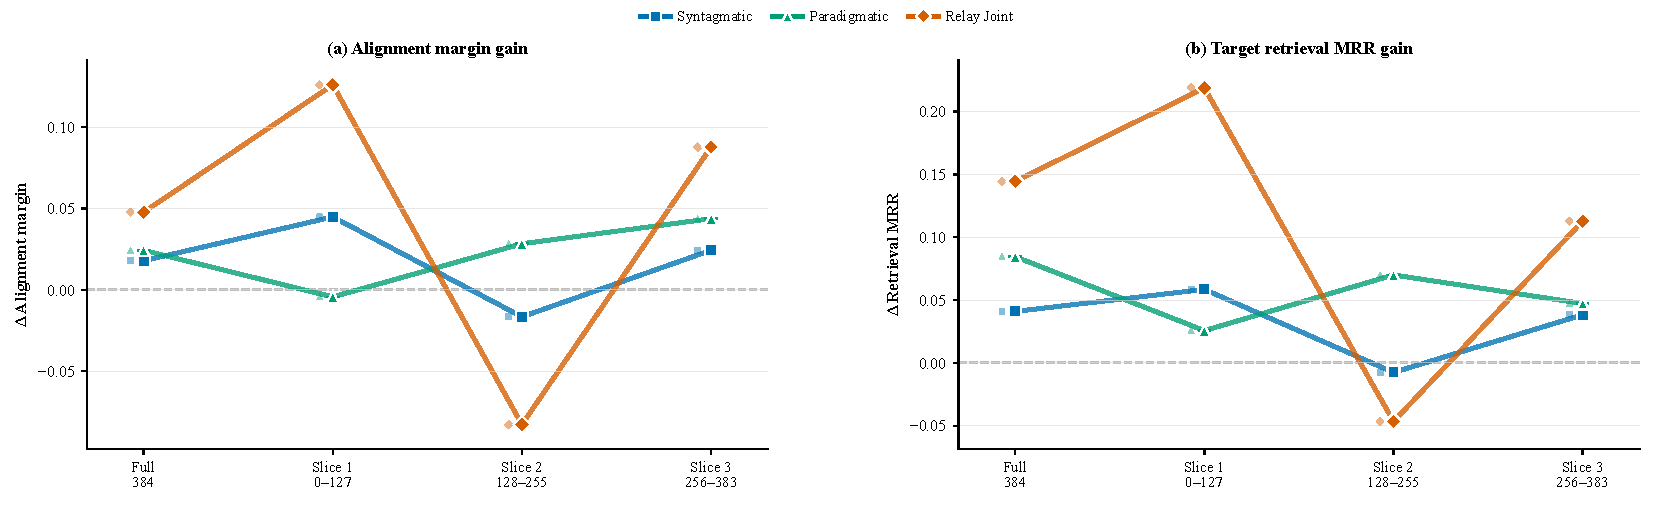
\includegraphics[width=\columnwidth]{figures/contextual_alignment_slices_v22_s0.pdf}
\caption{Seed-0 Paradigmatic neighborhood alignment differences from
Standard MLM for the exact 100M checkpoints. Full-384 is the primary
comparison. Relay Joint slice results diagnose its fixed training
coordinates. Points show the seed-0 estimate; no cross-seed error bars
are shown.}
\label{fig:contextual-alignment}
\end{figure}

\subsection{Syntagmatic Diagnostics}

The Syntagmatic probe maps the top-eight attention-selected
SentencePiece positions to gold Universal Dependencies words and also
removes those positions before the final Transformer layer. Table
\ref{tab:syntagmatic-diagnostics} compares only the models relevant to
this target.

\begin{table}[t]
\centering
\small
\setlength{\tabcolsep}{2.5pt}
\begin{tabular}{lccc}
\toprule
Method & Dep. R@8 & Dep. P@8 & $\Delta$NLL$_{\mathrm{att-mat}}$ \\
\midrule
\standardmlm & $.8737{\scriptstyle\pm.0059}$ & $.2990{\scriptstyle\pm.0018}$ & $1.3503{\scriptstyle\pm.4034}$ \\
\syntagmatic & $.8760{\scriptstyle\pm.0011}$ & $.2988{\scriptstyle\pm.0010}$ & $1.5793{\scriptstyle\pm.6814}$ \\
\bottomrule
\end{tabular}
\caption{Syntagmatic diagnostics, mean $\pm$ sample SD over three seeds. The final column is the attended-minus-matched increase in gold-token NLL under context removal.}
\label{tab:syntagmatic-diagnostics}
\end{table}

Dependency Recall@8 is slightly higher under \syntagmatic{}, while
Precision@8 is essentially unchanged. This does not show that the
attention target learns explicit dependency structure. Removing the
selected context harms prediction more than removing matched control
positions for both methods, confirming that the positions used to
construct the target are prediction-relevant. The difference is not
specific to Syntagmatic training because Standard MLM already exhibits
a large attended--matched gap.

\subsection{Interpretation}
\label{sec:discussion}

Relay Joint has the highest Overall in the seed-0 comparison, but the
two targets are not complementary on every category: Entity Tracking
and Reading decline relative to Standard MLM, and each single-target
system has task-specific strengths not retained by Relay Joint.
Attention-selected context is not explicit dependency structure, and
embedding neighbors are only distributed approximations to potential
alternatives rather than guaranteed grammatical substitutes. The
alignment probe verifies a narrow target-related property, not a
causal explanation of the downstream gains. The single available
Relay Joint seed further prevents conclusions about reliability or
statistical synergy.

% =================================================================
\section{Limitations}

\paragraph{Scope.} We evaluate only English BabyLM~2026 Strict-Small
and one 34.7M-parameter DeBERTa-v2 architecture. Most importantly, the
formal Relay Joint v22 checkpoint is available here only for seed 0.
The reported main comparison therefore has no cross-seed variance or
significance estimate.

\paragraph{Relational approximations.} Attention is not explicit
syntactic annotation, embedding neighbors need not be genuine
substitutes, and the fixed vocabulary-category rules are approximate
and English-specific. Fixed coordinate routing imposes a design choice
rather than discovering linguistic subspaces.

\paragraph{Results.} The seed-0 Overall improvement is modest relative
to the breadth of the evaluation, and metric directions are
inconsistent. Relay Joint loses on Entity Tracking and Reading.
Current evidence cannot establish that its advantage generalizes
across seeds, architectures, languages, or data regimes.

% =================================================================
\section{Conclusion}

We introduced Syntagmatic and Paradigmatic self-generated detached
targets for MLM without additional corpus data, external annotation,
or model parameters. Relay Joint stages the two signals with fixed
coordinate routing, reduced Syntagmatic retention after syntax-level
Paradigmatic activation, and a temporary entity anchor. Under the
fixed BabyLM~2026 Strict-Small exposure budget, the formal v22-s0
checkpoint reaches 40.94 Overall, 1.25 points above its seed-matched
Standard MLM baseline and above the two seed-0 single-target systems.
The largest gain is on BLiMP Supplement, with additional gains on
EWoK and GlobalPIQA, while Entity Tracking and Reading decline. These
results support relational representation targets as a promising
direction under limited exposure, but the single-seed evidence does
not justify claims of uniform improvement, significance, or general
synergy.

\FloatBarrier
\bibliography{references}

\clearpage
\onecolumn
\appendix

\section{Training Configurations}
\label{app:training-config}

Table~\ref{tab:primary-config} gives the relational settings saved
with the four seed-0 checkpoints. Onset is the fraction of completed
optimization steps. Standard MLM prediction always uses the complete
384-dimensional state. The two single-target systems also apply their
relational loss to the complete state; only Relay Joint uses fixed
coordinate slices.

\begin{table}[H]
\centering
\small
\setlength{\tabcolsep}{2pt}
\begin{tabular}{@{}p{0.13\textwidth}p{0.15\textwidth}p{0.17\textwidth}p{0.17\textwidth}p{0.18\textwidth}p{0.12\textwidth}@{}}
\toprule
Method & Syn onset / weight & Para syntax onset / weight & Para content onset / weight & Relational rep. & Entity anchor \\
\midrule
Standard MLM & Off & Off & Off & -- & Off \\
Syntagmatic & $0.0920386562$ / $5\!\times\!10^{-4}$ & Off & Off & Full 384 & Off \\
Paradigmatic & Off & $0.5522310170$ / $5\!\times\!10^{-5}$ & $0.99$ / $10^{-6}$ & Full 384 & Off \\
Relay Joint & $0.0920386562$ / $5\!\times\!10^{-4}$ & $0.1840773125$ / $5\!\times\!10^{-5}$ & $0.99$ / $10^{-6}$ & Syn 0--255; Para 256--383 & $\approx9.2\%$--$60\%$ / $2.5\!\times\!10^{-4}$ \\
\bottomrule
\end{tabular}
\caption{Saved relational configurations. After Relay Joint activates
syntax Paradigmatic supervision, its Syntagmatic weight at eligible
syntax positions is retained at 10\% of the earlier value.}
\label{tab:primary-config}
\end{table}

Both targets use $K=8$ and temperature 1.0. Syntagmatic takes
attention from the last layer. Paradigmatic has zero weight for entity
and reading-sensitive categories and no post-onset ramp. Relay Joint
does not enable a content projection or learned router. Its routing is
a fixed coordinate selection, and its anchor has no trainable
parameters. The total parameter count is 34,677,952 for every system.

\begin{table}[H]
\centering
\small
\setlength{\tabcolsep}{4pt}
\begin{tabular}{p{0.20\textwidth}p{0.72\textwidth}}
\toprule
Objective & Eligible MLM-selected positions \\
\midrule
Syntagmatic & Gold-token category is syntax, reading, or content. Entity and invalid tokens are excluded. \\
Paradigmatic, syntax & Gold token matches the fixed syntax list. It begins at progress $0.5522310170$ in Paradigmatic and $0.1840773125$ in Relay Joint, with weight $5\times10^{-5}$. \\
Paradigmatic, content & Gold token is classified as content; active after progress $0.99$ with weight $10^{-6}$. Entity and reading categories receive zero Paradigmatic weight. \\
Entity anchor & Relay Joint only: gold token is classified as entity; active from progress $0.0920386562$ through $0.60$ with weight $2.5\times10^{-4}$. \\
\bottomrule
\end{tabular}
\caption{Eligibility for the relational objectives and Relay Joint
entity anchor. Categories are fixed gold-token ID lookup tables
constructed from the tokenizer vocabulary before training.}
\label{tab:token-eligibility}
\end{table}

\paragraph{Vocabulary-derived token categories.}
No POS tagger or NER system is used. The tokenizer vocabulary is
scanned once before training. One recognized leading SentencePiece,
byte-level BPE, WordPiece, or space marker is removed; trailing
punctuation is stripped; and fixed-list matching is case-insensitive.
Byte tokens and entries with no alphabetic character are invalid.
The lookup then assigns the first matching category in this order:
syntax, reading-sensitive, entity, and content. Thus the categories are
mutually exclusive even when lexical lists overlap. An entity is a
remaining entry containing a digit, or an alphabetic entry of at least
three characters that begins with an uppercase letter. Remaining
alphabetic entries are content tokens.

\paragraph{Fixed lexical lists.}
\textbf{Auxiliaries:} is, are, was, were, be, been, being, am, do, does,
did, have, has, had, can, could, will, would, should, may, might, must,
shall, ought, need, dare, used.
\textbf{Determiners:} a, an, the, this, that, these, those, some, any,
all, each, every, many, few, no, much, more, most, several, both,
either, neither, such, what.
\textbf{Pronouns:} he, she, it, they, him, her, them, his, their, its,
we, us, our, you, your, i, me, my, myself, yourself, himself, herself,
itself, ourselves, themselves, one, ones.
\textbf{Negation:} not, n\textquotesingle t, never, no, nor, neither.
\textbf{Prepositions:} in, on, at, by, with, from, to, of, for, into,
onto, over, under, near, about, between, through, during, without,
within, along, across, behind, beyond, toward, towards, upon, among,
amongst, beside, besides, against, around, before, after, above, below,
off, up, down, out.
\textbf{Conjunctions:} and, or, but, because, although, if, when, while,
before, after, since, until, unless, whereas, so, yet, than, as, though,
whether, once, till, lest, except, provided, given, suppose, assuming,
whenever, wherever.
\textbf{Wh-words:} who, whom, whose, which, where, why, how, what,
whatever, whichever, whoever, however, wherever.
\textbf{Comparatives:} more, less, fewer, better, worse, bigger,
smaller, higher, lower, longer, shorter, older, younger.
\textbf{Temporal expressions:} now, then, ago, later, earlier, soon,
already, still, yet, finally, eventually, previously, formerly,
currently, recently, lately, immediately, suddenly, gradually.

\paragraph{Gold-token and context handling.}
Target-position eligibility is looked up from the clean gold/original
token ID, never the corrupted input. The same category therefore
applies whether an MLM-selected token is replaced with \texttt{[MASK]},
a random token, or left unchanged. The Syntagmatic context set excludes
padding, \texttt{[CLS]}, \texttt{[SEP]}, \texttt{[MASK]}, the target
itself, and every other MLM-selected position. Context embeddings are
then gathered from the original uncorrupted token IDs. Subword entries
are classified independently; the code performs no word reconstruction.

\section{Reproduction Mapping}
\label{app:reproduction}

Table~\ref{tab:model-mapping} maps each paper name to the exact seed-0
model directory used in the main comparison. All reported final scores
use the \texttt{chck\_100M} checkpoint inside that directory.

\begin{table}[H]
\centering
\small
\begin{tabular}{lp{0.70\textwidth}}
\toprule
Paper name & Exact model directory \\
\midrule
Standard MLM & \texttt{bb26\_claim\_clean\_s0} \\
Syntagmatic & \texttt{bb26\_claim\_comp\_entguard\_s0} \\
Paradigmatic & \texttt{bb26\_claim\_agg\_synonly\_s0} \\
Relay Joint & \texttt{bb26\_claim\_compagg\_v22\_v15\_relay\_synp050\_synkeep010\_s0} \\
\bottomrule
\end{tabular}
\caption{Paper-to-directory mapping for the seed-0 comparison.}
\label{tab:model-mapping}
\end{table}

Each model directory contains its saved training command, trainer
copy, and claim manifest. Evaluation results use the BabyLM evaluation
pipeline at commit
\texttt{3d57ddc8c40ee795c0b5e41b3a20251a9457a593}. The local evaluation
repository contained uncommitted changes when this version was
audited, so the hash identifies its HEAD rather than a clean checkout.

Figure~\ref{fig:reading-aoa} is generated from the official checkpoint
results for the four directories above. Figure
\ref{fig:contextual-alignment} uses the exact 100M checkpoints and the
new seed-0 CSVs listed in the accompanying v22 analysis directory.

\section{Representation Analyses}
\label{app:representation-analysis}

\paragraph{Paradigmatic neighborhood probe.}
The probe uses 2,000 eligible masked syntax-token instances. For each
instance, the correct candidate is the centroid of the eight nearest
input-embedding neighbors of the gold token. Sixty-three centroids from
other syntax-token IDs form controls. Alignment margin measures the
cosine advantage of the correct target over controls; MRR is its
reciprocal rank. Table~\ref{tab:para-probe} reports paired item-level
differences from the exact seed-0 Standard MLM checkpoint. Full-384 is
the primary comparison; equal-width slices are diagnostic coordinate
views.

\begin{table}[H]
\centering
\small
\begin{tabular}{lrr}
\toprule
Method / representation & Margin $\Delta$ & MRR $\Delta$ \\
\midrule
Paradigmatic / Full-384 & .024213 & .084507 \\
Relay Joint / Full-384 & .047681 & .144508 \\
Relay Joint / Slice 1 (0--127) & .125988 & .218807 \\
Relay Joint / Slice 2 (128--255) & -.082908 & -.046663 \\
Relay Joint / Slice 3 (256--383) & .087723 & .112787 \\
\bottomrule
\end{tabular}
\caption{Seed-0 neighborhood-alignment differences from Standard MLM.
No cross-seed standard deviation or significance test is available.}
\label{tab:para-probe}
\end{table}

The final 128 coordinates are the fixed Paradigmatic training slice
for Relay Joint. Their positive diagnostic values show alignment in
that designated coordinate range, but do not imply that the model
discovered an intrinsic linguistic subspace.

\paragraph{Syntagmatic diagnostics.}
Attention is ranked over SentencePiece positions before word-level
mapping. Selected subwords are mapped to Universal Dependencies words,
with duplicate words collapsed. Recall@8 is the fraction of gold direct
dependency-neighbor words recovered; Precision@8 is the fraction of
unique mapped selected words that are direct dependency neighbors. For
context removal, the same selected token positions are zeroed in the
input to the final Transformer layer. A matched control removes the
same number of random non-special, non-target positions. Tables
\ref{tab:dependency} and~\ref{tab:context-removal} include only the
current Standard MLM and Syntagmatic runs.

\begin{table}[H]
\centering
\small
\begin{tabular}{llrr}
\toprule
Method & Seed / summary & Recall@8 & Precision@8 \\
\midrule
Standard MLM & 0 / 1 / 42 & .8707 / .8806 / .8699 & .2997 / .3003 / .2970 \\
 & Mean $\pm$ SD & $.8737\pm.0059$ & $.2990\pm.0018$ \\
Syntagmatic & 0 / 1 / 42 & .8750 / .8759 / .8772 & .2999 / .2979 / .2987 \\
 & Mean $\pm$ SD & $.8760\pm.0011$ & $.2988\pm.0010$ \\
\bottomrule
\end{tabular}
\caption{Dependency alignment by seed and sample mean $\pm$ SD.}
\label{tab:dependency}
\end{table}

\begin{table}[H]
\centering
\small
\begin{tabular}{llrrr}
\toprule
Method & Seed / summary & Attended & Matched & Difference \\
\midrule
Standard MLM & 0 / 1 / 42 & 1.6525 / 1.6137 / .9038 & -.0447 / .1678 / -.0039 & 1.6972 / 1.4459 / .9077 \\
 & Mean $\pm$ SD & $1.3900\pm.4215$ & $.0397\pm.1128$ & $1.3503\pm.4034$ \\
Syntagmatic & 0 / 1 / 42 & 1.8058 / 2.1002 / .7960 & -.0438 / .0159 / -.0082 & 1.8496 / 2.0842 / .8042 \\
 & Mean $\pm$ SD & $1.5673\pm.6840$ & $-.0120\pm.0300$ & $1.5793\pm.6814$ \\
\bottomrule
\end{tabular}
\caption{Gold-token NLL increase after context removal, by seed and sample mean $\pm$ SD. Difference is attended minus matched.}
\label{tab:context-removal}
\end{table}


\end{document}
